\documentclass[12pt,letterpaper]{article}

% --- Paquetes Básicos ---
\usepackage[utf8]{inputenc}
\usepackage[spanish,es-tabla]{babel}
\usepackage{geometry}
\geometry{top=2.5cm, bottom=2.5cm, left=3cm, right=3cm}
\usepackage{graphicx}
\usepackage{booktabs}
\usepackage{amsmath}
\usepackage{amsfonts}
\usepackage{float}
\usepackage{caption}
\usepackage{subcaption}
\usepackage{fancyhdr}
\usepackage{hyperref}
\usepackage{listings}
\usepackage{xcolor}

% --- Configuración de Hipervínculos ---
\hypersetup{
    colorlinks=true,
    linkcolor=blue,
    filecolor=magenta,      
    urlcolor=cyan,
    pdftitle={Informe Tecnico SmartHome IoT},
    pdfpagemode=FullScreen,
}

% --- Configuración de listings (Código Fuente) ---
\definecolor{codegreen}{rgb}{0,0.6,0}
\definecolor{codegray}{rgb}{0.5,0.5,0.5}
\definecolor{codepurple}{rgb}{0.58,0,0.82}
\definecolor{backcolour}{rgb}{0.95,0.95,0.92}

\lstdefinestyle{mystyle}{
    backgroundcolor=\color{backcolour},   
    commentstyle=\color{codegreen},
    keywordstyle=\color{blue},
    numberstyle=\tiny\color{codegray},
    stringstyle=\color{codepurple},
    basicstyle=\ttfamily\footnotesize,
    breakatwhitespace=false,         
    breaklines=true,                 
    captionpos=b,                    
    keepspaces=true,                 
    numbers=left,                    
    numbersep=5pt,                  
    showspaces=false,                
    showstringspaces=false,
    showtabs=false,                  
    tabsize=2
}
\lstset{style=mystyle}

% --- Encabezado y Pie de Página ---
\pagestyle{fancy}
\fancyhf{}
\lhead{SmartHome IoT - Informe Técnico}
\rhead{Equipo 69}
\lfoot{Universidad de Talca}
\rfoot{\thepage}
\renewcommand{\headrulewidth}{0.4pt}
\renewcommand{\footrulewidth}{0.4pt}

% --- Inicio del Documento ---
\begin{document}

% ==========================================
% PORTADA
% ==========================================
\begin{titlepage}
    \centering
    \vspace*{1cm}
    {\includegraphics[width=0.35\textwidth]{logo_utalca} \par} % El usuario puede subir el logo a Overleaf
    \vspace{1cm}
    {\scshape\LARGE Universidad de Talca \par}
    {\scshape\Large Facultad de Ingeniería \par}
    {\scshape\large Escuela de Ingeniería Civil en Computación \par}
    \vspace{1.5cm}
    {\huge\bfseries SmartHome IoT: Sistema de Automatización, Monitoreo y Control de Acceso para una Casa Inteligente\par}
    \vspace{1cm}
    {\Large\itshape Informe Técnico - Proyecto Unidad 1 (Equipo 69)\par}
    \vspace{2cm}
    {\large\textbf{Integrantes:}\par}
    {\large Mariano Muñoz R. \par}
    {\large Cristian Ruiz I. \par}
    {\large Camilo Fuentes G. \par}
    \vspace{1cm}
    {\large\textbf{Profesor:}\par}
    {\large Ricardo Pérez \par}
    \vfill
    {\large 9 de Junio de 2026 \par}
\end{titlepage}

\newpage

% ==========================================
% ÍNDICE
% ==========================================
\tableofcontents
\newpage

% ==========================================
% 1. INTRODUCCIÓN Y DESCRIPCIÓN DEL PROBLEMA
% ==========================================
\section{Introducción y Descripción del Problema}

\subsection{Introducción}
El desarrollo del Internet de las Cosas (IoT) ha revolucionado la forma en que interactuamos con nuestros entornos cotidianos. La domótica, o automatización del hogar, ya no es un concepto futurista exclusivo, sino una realidad accesible que permite integrar sensores, actuadores y algoritmos de control para mejorar significativamente tres pilares fundamentales de la vida moderna: la seguridad física de los habitantes, el confort térmico y ambiental del espacio habitable, y la eficiencia energética mediante el control inteligente de recursos.

En este proyecto, se diseña e implementa un prototipo completo y funcional de casa inteligente. A diferencia de las soluciones comerciales cerradas, este sistema se fundamenta en un diseño distribuido y modular que combina hardware de desarrollo real (Arduino MKR1000 y ESP32-CAM), protocolos de comunicación estándar en la industria (MQTT), una plataforma visual para lógica y paneles de control local (Node-RED), y una capa intermedia de visión artificial con base de datos dedicada (FastAPI + SQLite) para la autenticación biométrica de accesos.

\subsection{Descripción del Problema}
El caso de estudio involucra a una familia que desea automatizar su residencia debido a diversas necesidades cotidianas insatisfechas. En primer lugar, la seguridad del hogar es una preocupación crítica: requieren un control de acceso automatizado en la puerta principal que permita identificar visualmente si hay una persona presente y autorizar la entrada únicamente si esta pertenece al núcleo familiar, registrando cada evento de acceso e identificando rostros desconocidos para su posterior enrolamiento. En segundo lugar, existe la necesidad de monitorear en tiempo real variables ambientales para asegurar el confort y la salud, específicamente temperatura, humedad e indicadores acústicos. Por último, se requiere un esquema de alerta temprana y automatizada ante anomalías críticas del entorno, tales como fugas de gas licuado o humos nocivos, que actúe de manera local activando alarmas visuales y sonoras, y de forma externa enviando notificaciones detalladas a los celulares de la familia para permitirles reaccionar oportunamente incluso si se encuentran fuera del hogar.

El prototipo desarrollado resuelve estas problemáticas mediante un diseño distribuido que integra hardware real de sensores y actuadores con contenedores virtualizados que simulan una infraestructura en la nube o servidor local dentro del hogar.

% ==========================================
% 2. OBJETIVOS
% ==========================================
\newpage
\section{Objetivos del Proyecto}

\subsection{Objetivo General}
Diseñar, implementar y evaluar un prototipo funcional de sistema IoT para la automatización, monitoreo ambiental y control de acceso biométrico de una vivienda inteligente, utilizando sensores físicos y actuadores conectados, comunicación por mensajería MQTT, procesamiento de imágenes por visión artificial y reglas de control en un panel visual integrado.

\subsection{Objetivos Específicos}
\begin{enumerate}
    \item Programar y conectar un nodo sensor/actuador basado en Arduino MKR1000 para leer de manera robusta variables físicas del entorno y controlar actuadores locales de alerta y acceso.
    \item Integrar una cámara ESP32-CAM al broker MQTT para transmitir ráfagas de imágenes JPEG a demanda ante eventos específicos del sistema.
    \item Establecer la comunicación de red inalámbrica mediante un broker MQTT Mosquitto centralizado, utilizando una jerarquía de tópicos consistente y estructurando la telemetría en formato JSON.
    \item Diseñar e implementar un flujo en Node-RED que actúe como panel de control principal (Dashboard) para visualizar datos históricos y en tiempo real del sistema.
    \item Desarrollar e integrar un backend en Python (FastAPI) con la librería \texttt{face\_recognition} basada en dlib para el procesamiento biométrico de rostros, controlando la apertura automática de la puerta y el enrolamiento temporal de desconocidos.
    \item Codificar estrategias de automatización basadas en umbrales de seguridad para alertas de temperatura, gas y sonido en Node-RED.
    \item Integrar notificaciones externas de mensajería (Telegram Bot) para el reporte instantáneo de emergencias y la recepción de comandos remotos.
    \item Registrar históricamente la actividad del sistema mediante un archivo plano CSV local y una base de datos relacional SQLite que garanticen la persistencia de datos.
\end{enumerate}
\newpage

% ==========================================
% 3. ARQUITECTURA DEL SISTEMA
% ==========================================
\section{Arquitectura del Sistema}
El sistema se diseña bajo un esquema de arquitectura distribuida y desacoplada, donde cada componente se comunica de forma asíncrona mediante el broker de mensajería MQTT. A continuación se detallan los aspectos lógicos y físicos de esta solución.

\subsection{Arquitectura General de Componentes}
La topología del sistema consta de cinco bloques principales coordinados a través de la red local:
\begin{enumerate}
    \item \textbf{Nodo Sensor (Arduino MKR1000)}: Lee periódicamente las variables de temperatura, humedad, gas analógico, gas digital y amplitud de sonido. Actúa de forma pasiva a la espera de comandos MQTT para activar el LED de alerta, el buzzer o el LED indicador de puerta.
    \item \textbf{Cámara IoT (ESP32-CAM)}: Se conecta por WiFi directamente al broker MQTT. Permanece en estado de reposo hasta recibir un comando en el tópico de captura, momento en el cual realiza una ráfaga rápida de capturas a alta velocidad, enviando los bytes JPEG directamente por MQTT.
    \item \textbf{Broker MQTT (Mosquitto)}: Contenedor Docker que actúa como el bus de datos central. Redirige los mensajes de telemetría y comandos con configuraciones de calidad de servicio (QoS) apropiadas.
    \item \textbf{Motor de Reglas y Dashboard (Node-RED)}: Contenedor Docker encargado de recibir la telemetría de sensores, actualizar el panel web de Node-RED Dashboard, evaluar umbrales críticos de seguridad, enviar notificaciones externas por Telegram y registrar las lecturas en un archivo CSV local montado en el host.
    \item \textbf{Servicio de Acceso y Visión (FastAPI Backend y Nginx Frontend)}: El backend en FastAPI procesa las imágenes de la cámara, realiza la comparación geométrica de rostros con encodings almacenados en una base de datos SQLite y publica comandos de apertura de puerta. El frontend (servido por Nginx) es un panel web alternativo especializado en el monitoreo del acceso de personas y el enrolamiento en caliente.
\end{enumerate}

Para visualizar la interconexión física y lógica de los componentes, consulte la Figura \ref{fig:arqui_general}.

\begin{figure}[!htbp]
    \centering
    \href{https://www.plantuml.com/plantuml/svg/XLRDRXit4BxlKmnyQ6N0YXmvDLmZABAIxDYjtIYMahO8Wc347Ib4Tac5v2fnYZnC7g2dt7hLYtL8IkkLjQfpY9Vazyt_VFOpwz2uiiWJ-q6gEHeiGEXYhXKfDtAtEG4_Tckl6JgSeAKUYWypeqkLzNMk3Lp9sNlt5-Mv_bH3et3QD49xUKareD9Piyd-BQeQxcD9PJFmkI5IYPEEOqxDnr8w4guq2Cz9aS4SCifX9AsZ0c5KSDeNkY2ur6De4SFd-lZd_IG437klR8b6QcZzZWkQOQRD_XwWXLUMp1PcJ3dDEBW8MPy2rAS5U_rSSZa9Eb2PWpzeiWT_9m1mLt3OksIOcU8N_mojSwFvhB9eU7rAv_FawyhoYCn2iZcoRFnIJGsITQQCYRS6MdmW0trltzB-sb_uRnLPC4biuHIcA_kSz4ogpt1wSbXHDiEit8Om0zf76B_y6vd0-lf_xYRSnE3j7ArBXvVUt-5EZsiG9nzSzIARZyreGKEZ1Lch3RIcV7ndIEYPaavg5UlfGMUAGwQrYMguESENLz8Hj51u8-y41svq_YYRHEwWzt22XRP-2XrFICzetuZJnoSdH_KCmpWpRVL-_N8yzkR3Hxnxs8s_CUIxnX_jcxE1TxExTHNgd3VL1c_-weQoXYgyvtNHHcB-IDX5mFP7hyzbJZ6iQWm7qlA4SMqNsW9VNA39Fg7X-bMBrZHzgSbAgJHS_tRpc7iV7F3tZWcGfl0sxwFNznMd-fZgd4lZfrLPRIYWGnIrVsz65-EZGx_3nRnpKHRxRxtPSBc9ktxPxaBhEJ-YmdpvVIQ5XXyWapFfC0yqRblt7YdzyycJusCkWrQyBvrhALR8-52Xl-wEFkLbncnd_5VSoZGdutZVXrB1SNJ0r-5s6pmixy0d5NYWjTd4zielNyX4t4yH5w_gGJSDvzbeUDHjzzFhqA5muiC3JTqazR7OQkkR_l8R3nF2YzVTuoU7RrSuCbWDeyXrcS7UMe712qOhIAeYjwdE_9Jy2Bn7YeIN19julOPs-vUwpi8f13eAj_oNQtOn7Wyxluxsapg6ENNbOywGd1Hib2nuHb9_PNHDl3pOwC_IwpVEPL9xOM1DeY9Ga4MGnVBRZDZuVVIWnwWheiwP5KPE2AhrXLieus-hBL8bDI7mSf9BWR2IkqvEMNiUv-KM1FhoTmJENSb5hn6VjjkREOtALGIuPia2EUOxAwN9avNkR8THesVej3rOisX1okc3JQCDTdQdSr0T9d6Ow-ILk37pXcPSEuEXXCllHWfjA-XJnjO7YV5dQh7y1m738d8lsO3m2V2eeygOM_-heCb0VSmuGkXfjydn5F_1s1SJ_hb06A1zFz5eiZj_QGmWgIrGOCP5OMu_TW-cXc-sSStbQsvXRCRzEQXRR1g4QdnOkUkUW-J6-UMTxVRtjn2ihkltz4w2qqDMuK5KOKYx3RGejKtKnrleIZTzgUAWyDglp3UYlN0sWGy0IwVRUZg58xlDZ5Bwi9UTJGcB0RTnvBQsqPjexiBkLJXeMFla6UzqMUJ_0G00}{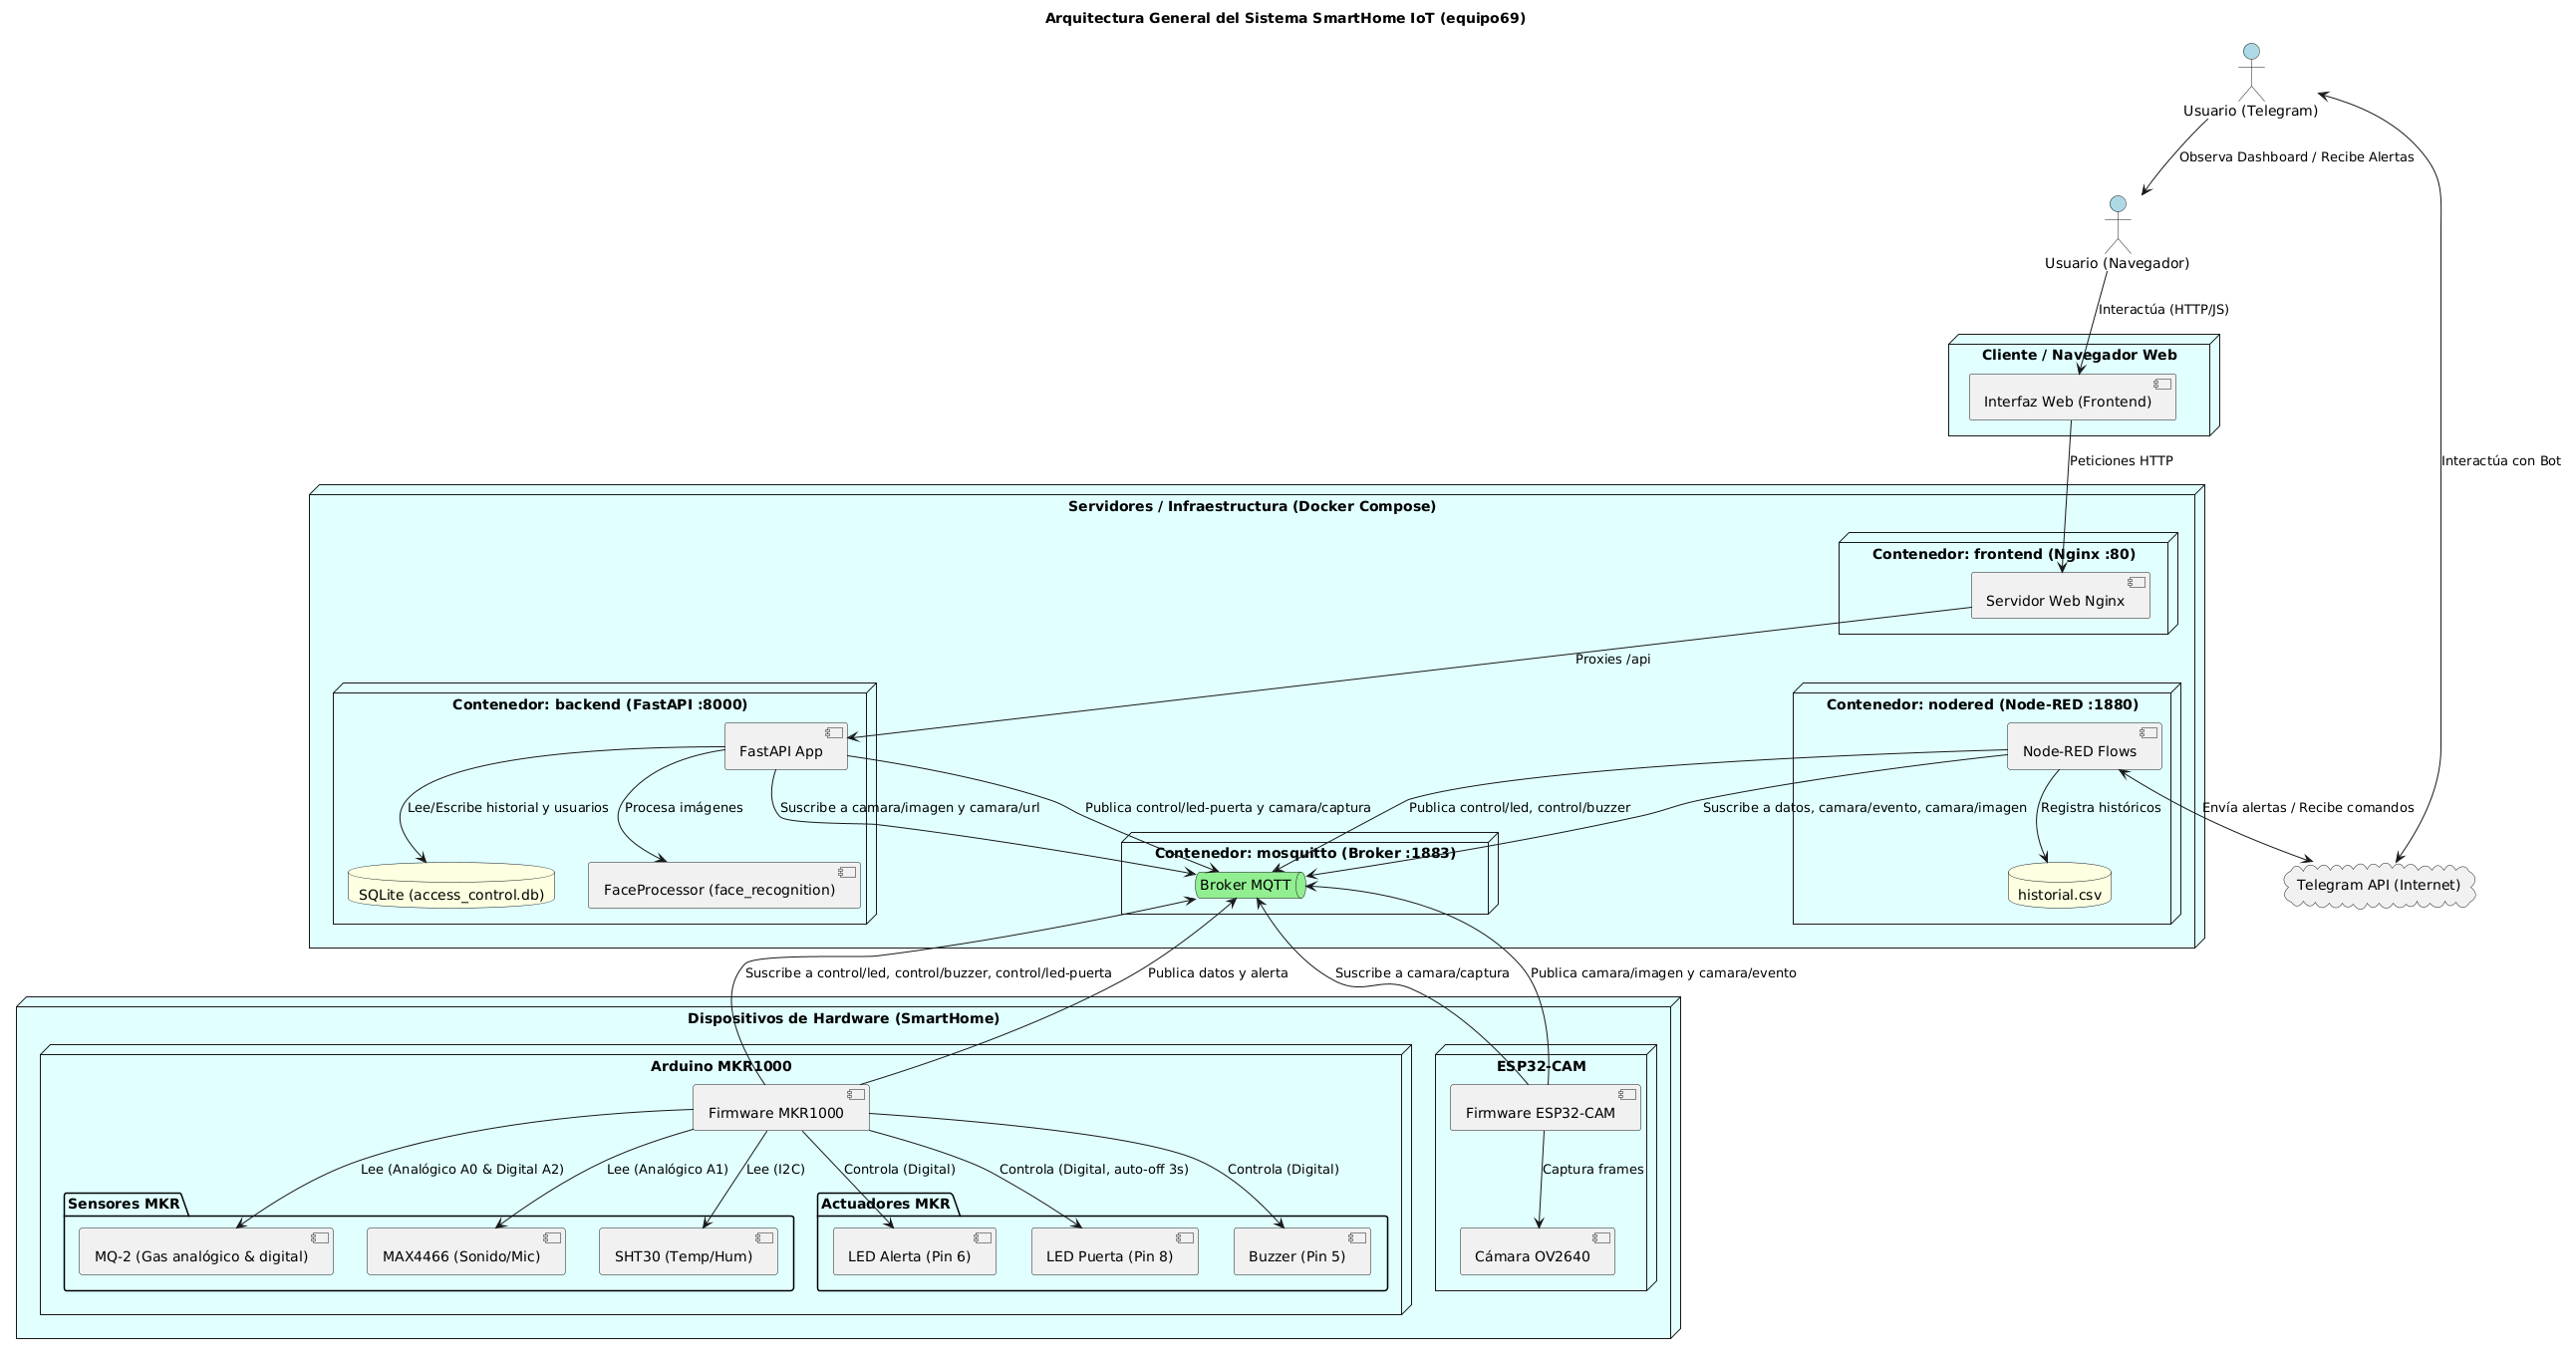
\includegraphics[width=0.75\textwidth]{arqui_1}}
    \caption{Arquitectura General del Sistema y Conectividad de Red (arqui\_1). Al hacer clic en la imagen se abrirá el SVG de PlantUML en alta resolución.}
    \label{fig:arqui_general}
\end{figure}

\subsection{Secuencia de Control de Acceso Biométrico}
El control de acceso por reconocimiento facial opera mediante una secuencia asíncrona optimizada para evitar la sobrecarga de la red local y proteger el hardware de la cámara. El flujo principal se detalla en la Figura \ref{fig:arqui_secuencia_acceso} y consta de las siguientes etapas clave:
\begin{itemize}
    \item \textbf{Activación}: El usuario solicita una apertura desde el panel frontend o el sensor de sonido detecta un ruido inusual. El backend FastAPI publica una orden de ráfaga (\texttt{iniciar\_burst}) hacia la cámara.
    \item \textbf{Captura y Transmisión}: La ESP32-CAM captura imágenes VGA de forma no bloqueante a una tasa fija de 4 frames por segundo durante 5 segundos (20 frames en total) y los transmite como bytes crudos de datos binarios mediante MQTT.
    \item \textbf{Procesamiento e Identificación}: El backend FastAPI recibe estos frames y los procesa en sub-ráfagas de 3 segundos mediante hilos de ejecución paralelos con \texttt{face\_recognition}. Si se encuentra una cara conocida con una confianza mínima de 50\% y una tolerancia estricta de 0.35 en al menos 3 frames consecutivos, se concede el acceso.
    \item \textbf{Apertura de Puerta}: Al autorizar el acceso, se guarda el evento en la base de datos SQLite como ``Entrada Automática'' y se publica la orden de encendido de la puerta por MQTT. El Arduino MKR1000 recibe esta orden, enciende el LED físico de la puerta y ejecuta un temporizador local no bloqueante de 3 segundos para apagarlo automáticamente.
    \item \textbf{Enrolamiento}: Si no se reconoce el rostro, el backend guarda el evento ``Desconocido Detectado'', extrae y almacena temporalmente el frame en caché, y abre una ventana de enrolamiento de 60 segundos. El frontend detecta esta condición mediante polling al endpoint de eventos, activa un temporizador visual y permite al usuario registrar al visitante escribiendo su nombre, guardando su encoding en la base de datos de manera definitiva.
\end{itemize}

\begin{figure}[!htbp]
    \centering
    \href{https://www.plantuml.com/plantuml/svg/hLTTRYEv4NxlKnGwG20XOrcsuGKoW1ShsRAZMVze9Sq6GJOGIjqbcPbkiaEoFUDT6CWXSe5vt8SvXM-IawJOLDDkj-NvGHvsHoRh--fZ_HJPFnYBsfPv1gZ_LOh5VXHXQPKiyoNfoBmJia2DEGpLXmccgP1hsEi_MfymMYIYG6aVxKTMs8nWHab9CX7u6gQKAAaIaGkILi4fyce6jt2ifDKgWvHWa2Ha57I8THJgkpztesYfFa1ygjc6P0f_XBUcH2rK37yu5-jhEynAYW00CB5AGnosqR0fwMglU508yINUq1fJDluhBN-HdR_CByvttyow5QHs53bdx7hZVuZ9E-z-Y8QSqXEqojGY_aPPfjwtNPsYiOF960P5mOwm4BjQbPPChxZrxdZpELH24wqu4aPfnXNrxm2hBIfiYXQNJbKy--bSM7AU4WTO93wmlNJfOIV3fyVIwXrfFjLOpU5IfHHETAQ9P5lQXJAS6MiLU2ZxklXfFlVqVgaD6iqc1_ixnuCBjZuLEd-FcZpY67FdjGqPwBGKKi75ZzEzVh_V0l9w1Gp7EJg2lHwS2CCq2b9YwiAM6e5WB9csMflUVrpX6k7eA7Ab0JlVXtp3QvXeCa99XFXdtXldk2OPmsxD50LJXhcaCk9gDeTTbzR4ssZWQffFkX4cLjoWfIh1aRDca8-FmvNBJ2G89aTjhrLEktMzCn6lOSttY_mjvbooglWrnC8T1FLYMMfZurSGfsoosJoyYpmzEwh3ofukI1hy9u5B4cXAn5AaAgWByQy13Ip_MWe4CXPJ1GYp-M0-MWpVJcVpyULP56LA5MoK8kmVzdC3JeraqaCmj2vbgaoLrotSFZkd6dE2DvFH6NH-FXjqcuYl2fce4WP_hyY6jvRCFnnRJH6IDf9M4nV1WnrW5P_ZpCsb2kCi0s2GvPYGH5XLOjd7ibojc98bteYKbAl2AALML5rHxlV0jp9MKwzHXhTF9-BHaGzg4r4e3QPSxcWFCz19ND0FJDTfsKocHxB3T63jcz7XIwPJ7S0il7mVwo2wCL82GvED1_MD8CtMdWaGfcT3810fAnKhbo2jZEN_MZGdGoPOarrWbYrAGzfqkj2vMbf1qWKrKUxYCE03miNZzJ5ifodYN1YBa3x6kDjAYr-HKI_Bpzs5zGZOcQkCDBhhwQZVEpXyvOwu4YX_nUzvuR3lHVX8PHQE1xCh63WcmPYK71167uHL1g5pSVz9zk2W3exhWeU3D7M5ulejzltb-hiWdGlB4DVRfR_7tFgR4kMZfOL8UNNlBj2cz7mMwvAeeo-a8MqNTCF9wiIk3rmT3JXu-Vr7oybZ9my-ZlOUX7_D0FDtpcv6wKvHihydG-pgClRAcxt90_sbaHKGzKbhGBqH21fS8quGIVuv6LykpaSdYydRqNG-WCwaKWQu5ExVxeii_W91i2BtJNyG1jot1AYwczMkJpl7vaiBuAxfh7btJSaKoXrqlz-7gn_X6rW3cwDsrwFBHSaq6Y7UlCicDHNyzz__WOe0RbrEIiou_-1Q6DU9c0NMyAFNu-kPLPRtlvjc4DtMomb8hYbvTwAKFgTqpbbGfUrqgm5Tk3dQJ6wxBTh5qcpe8SUlcbfEO3r_-BUbn6AelQrZPKOPkV8EDmHJWFQ4t5W6rXevDP-ZQLypEUKkc91WSdt_--Vm9xGIac15oJL2Tl-94qL-J6gLrNT9Hwhty2Vuhl_bKoabIMjyMZsop39UgBJodquYfOlgpxil63xF1Zhk_X_xQRjqNWxEkVw_tQMFh6xEjysYSsb5xhJaXLiVwuMy_75wDlxU7iYlgw9JpoFx-5suSSL6NCyVTQmtEf9Sz23qUEQIkaP5dxEyIPATDkkt1uUDohBt2TYKhqScwEq_SG-6srUs6N6uLGxLVseBQyTzxoeuf_bRBLWxIcxeautsbBdKx9AiyRQ4em03jRzHt_FgEWpQUByU46SY2qrpSdoad2P4PjPNP9RQyjq73mAkK1SuAFWhk4wP7EbT5vchWXQJNuBYIgbJTLxkOd-SvyxOxdMP12aofUQe1DFADNSWmmlmfVGQ5FDBtxya3VYO7WkTn1FTlVizr0xSJuQGKBKVizi6NfJIig2T3qq7tKsSsu69n-8FbYD3o_6mFPqEfNy_rh5gs2-M6PgsOtQJr5dlX3fDd7d8Y_2-6Pj6v6teToYTaa6pkSUTLyqC4GQ1vPNq4x9avRULcTN2NVSIsKMFJTh1XbfHdbV6_DKGQAqTltWwftYAFg1OMMUHT7_0000}{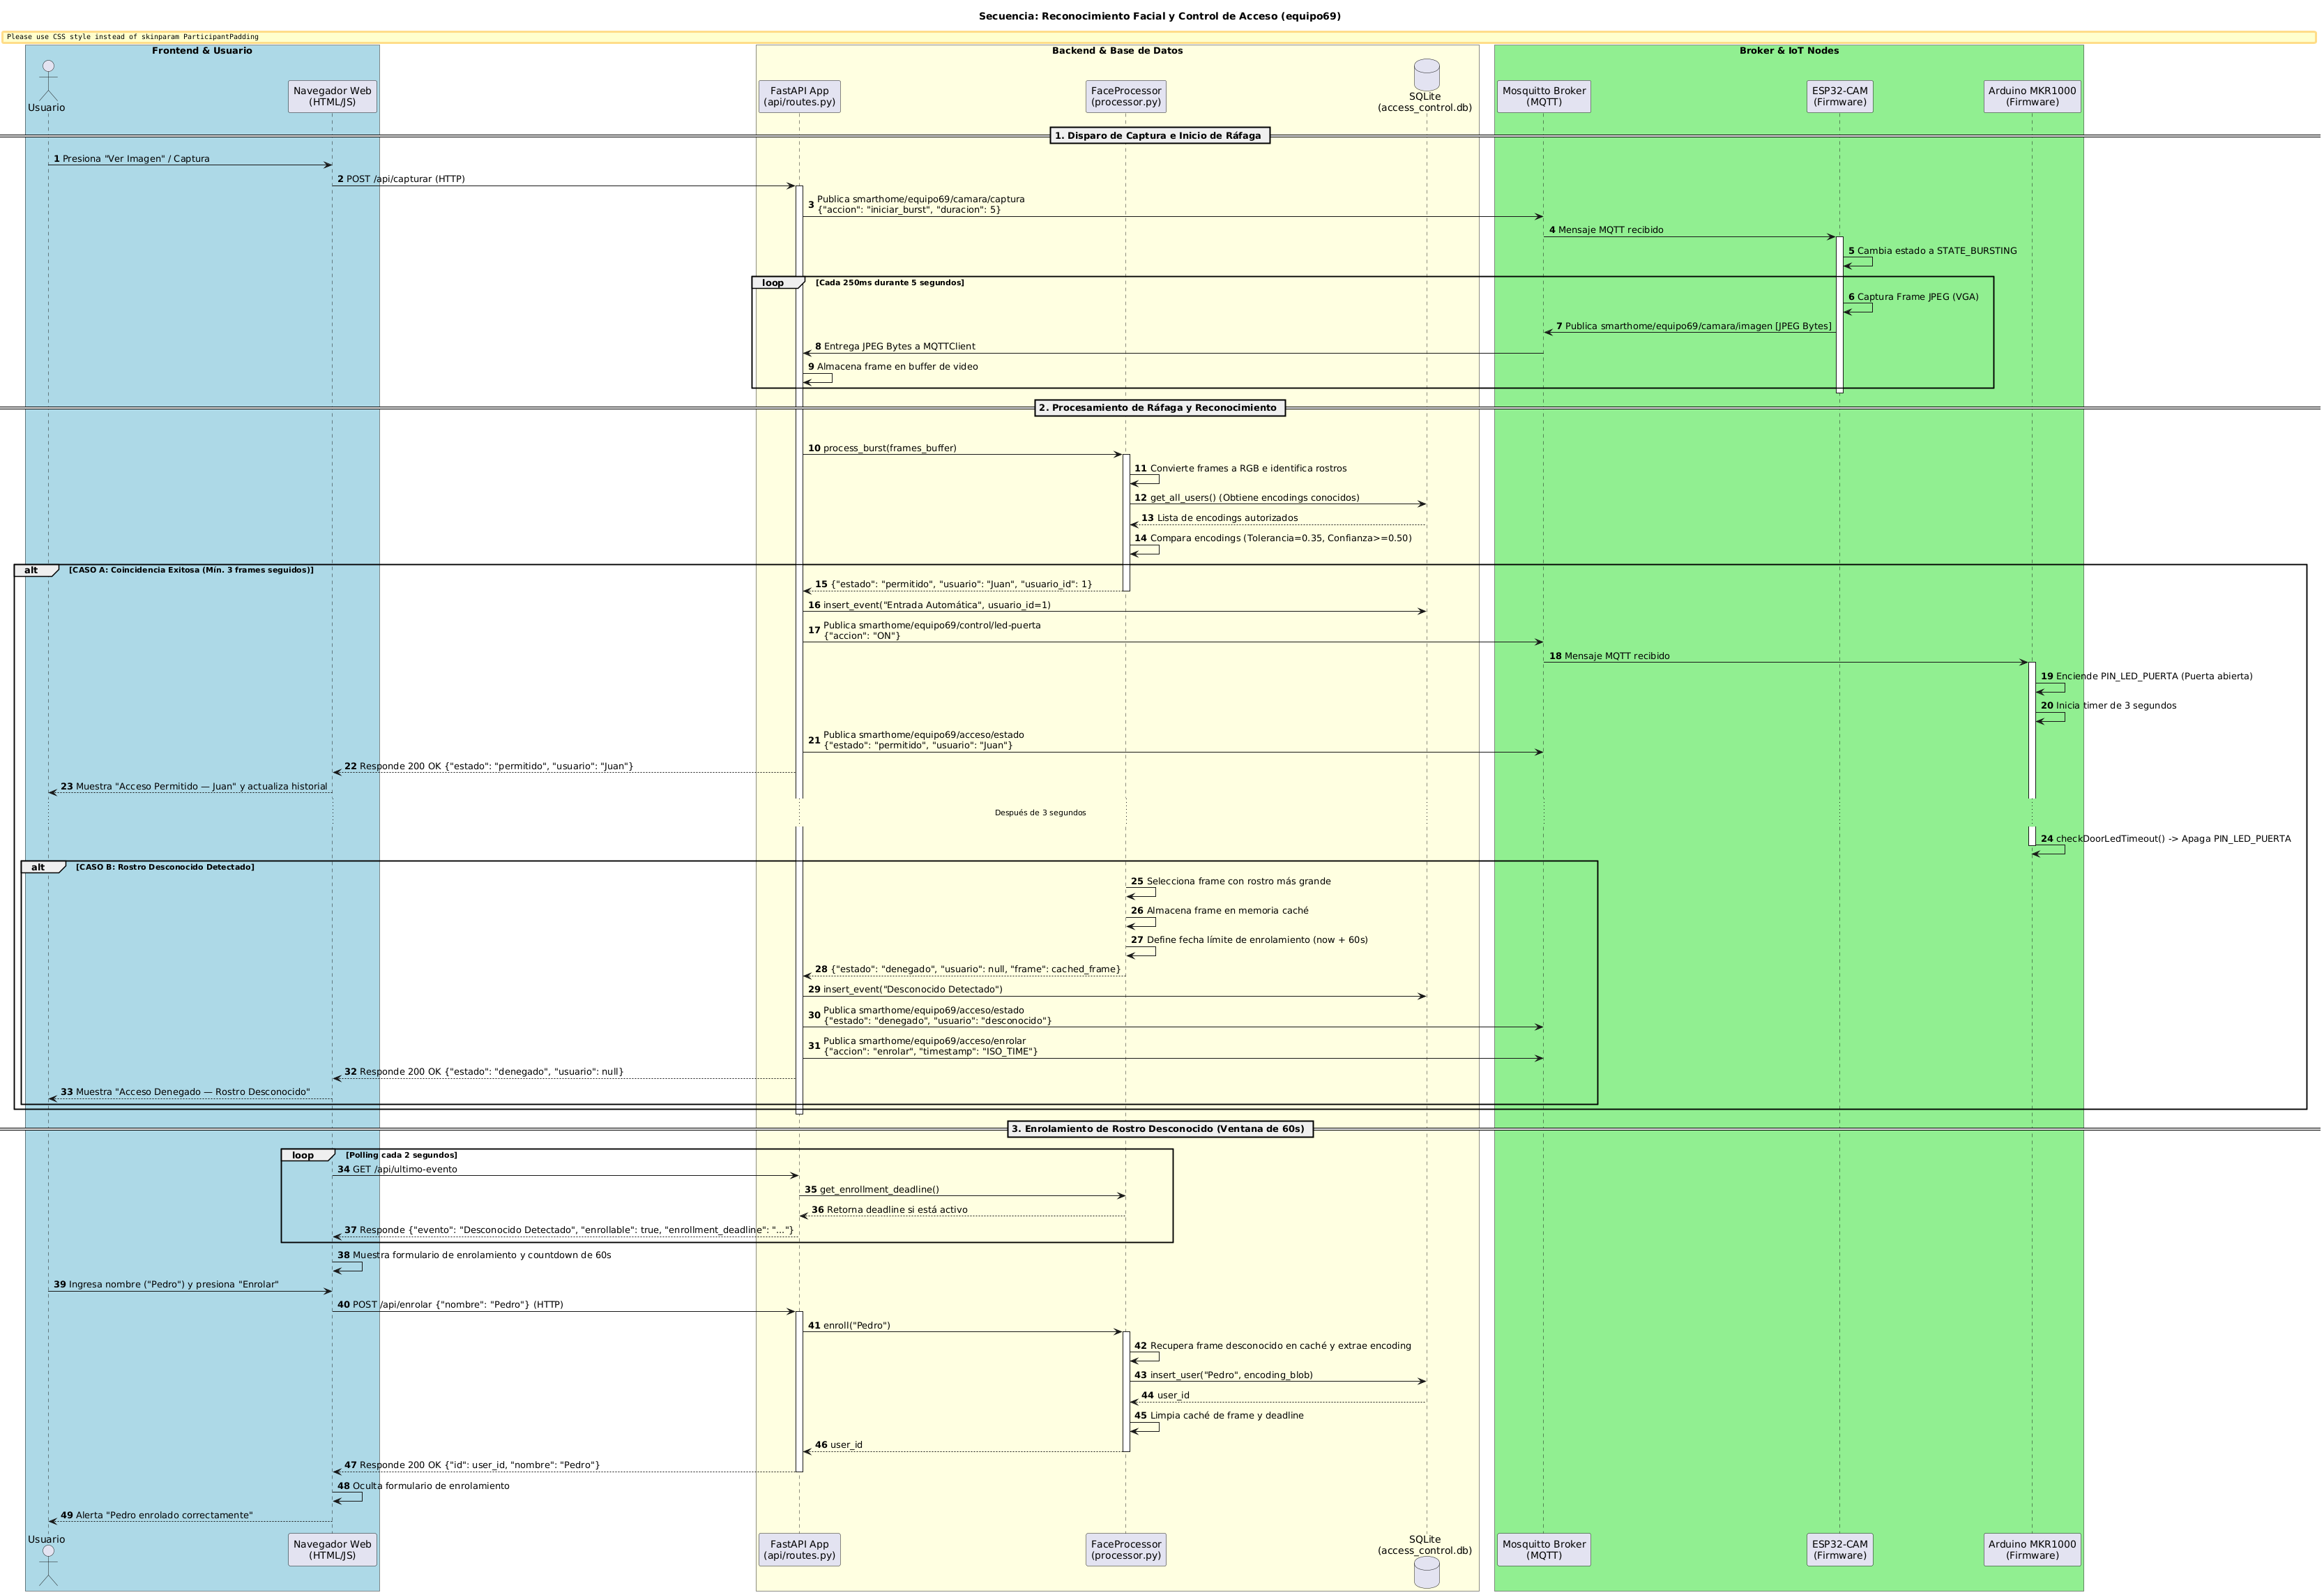
\includegraphics[width=0.75\textwidth]{arqui_2}}
    \caption{Diagrama de Secuencia de Control de Acceso y Enrolamiento Facial (arqui\_2). Al hacer clic en la imagen se abrirá el SVG de PlantUML en alta resolución.}
    \label{fig:arqui_secuencia_acceso}
\end{figure}

\subsection{Secuencia de Monitoreo y Reglas de Control}
El monitoreo ambiental y las reglas de seguridad automáticas se ejecutan de forma paralela e independiente en Node-RED. La Figura \ref{fig:arqui_secuencia_telemetria} describe el flujo desde que los sensores físicos leen las variables ambientales hasta la activación de alertas y notificaciones. 

\begin{figure}[!htbp]
    \centering
    \href{https://www.plantuml.com/plantuml/svg/rLPFRnl56xxlftYrF-cdH78SnqahrP9BdTHD2eaRR8D0RHMztdcx6JexOsPctJ-88nUkt10IwerB9IHkN92QRy8du2FmpWoRE2vGQ90GbsJNy_v_dkUTlUKyMbzN2j1-MikJxIp3sXjTLpEoMUQbLmGJAchIXSGUJ4bHHTwUlSGM3DYoGY-VOo7FVj3m30QAh4S7QyJ1vkRwZVKicvcda1-W5K_G4jmrqnp-ToZBKx-hQie00EPSWYpa7BM7V615BRM1e_V6MvrE9mTquVbrm-7aUBkxiJSuYYRybf4MmDb-IxbhpMEoSFJ-z3pZlYNIhqSwCexBzTv0yea1q-DAp94Hj34UteR_SwiL5gInagIzQJ9yJ4gP9wifbXplyB6B2KQf9u4UP-W8ybFflB4ILRjmYsYoD_bmfO0ZqWu_eJ1_63xrP3KsgO-bVlnwuW1OQR62mV7T67Ew7usmu5oGV-1gjD90OvRIgj3JHUP-7xRQCDIBivS612sJ0DRsK21qmL5PQs7SElJxcJ9c3kc08OJAnPIC8cpSZFzwS4W4auFfTgV526rq-U_WevsTwzUNBHC4R7nSpvGi45p5hPsQYZORVcto-8nxe3_BFLLpikXhYtblsk9nrXK957dlW5zAT7blFpsS25bAZohlvUrsE-SV7K_Ls1DwweFpvFDGH9ETwnXnmTo-jrGYL0a1U7ToRnJjHh5MXegDzdcQ0e4qXC9mynAa3_HzBojo7gjv2xX4BenBchG0esmUDk6Qb8F2rwXONh2FTKcEpUtPYqUoC8wrja0EF5Fae5HcXlmG48jeTHcj1QewwJ90DgPIeGFMdsPgH1GRhJ9Ug7ooW2sM-CKWuIPiT-3LztkfihyCIc5uM4PjAXAGtnlbR-a-gvy_9xiQOReFlKH6XDG32BfKzTpOSq97HtPXnqHhTauYeXxaltpxzNTmVn9AEE0IO70u74y73oz5AvZddYiDN5aXHgBoK1SSc6iu7DvkAdeM12ON2BknXuoKIo0WT9acw7YqMvrk1-RpwjySxbj5GFuD-Tyyp2Te3mlcb6OzoS0kj2UpsZgVjtB11kdesggeU65pcZ4LSaRWhInBia2G8a3WEPOHsKU65Vv6_7caLyTz9PuWJuL7yOz1lzs3YT5I65XRNZdhWGpNEh0shgLOqkRwVm6OPkTijwDgZELz9OoDNSonvEVqdN3sWaN4ZH-YBqxvb3k68wbhltnd76CG70e4HKLKdpQsGWNCMaT57UTA6fhhT7LZllffw3mkpn3wS6y4pvfu3b90Skz4tx3vfXQrAsfhUVYio_vIPR1sezDffJji7PpKe6jQeBi8rso7nD2LSXI94wx74_HPQ7Vk919THUvNYv4qln9cXTC9jSk45kGkSJhwCl3duE-q-MBnPB58Dmud15AmQppxdciom9p4kAhZmbIe6RRDCAtQPNnsVkyks3u2sjoyDb2JiSgM9dr816S_AYyhT4itO_Ig3Bz2kYIpfHqo9ZStMb2izXnGqk1b83BdOVi_MI5VVGaN6sGI2q-tPx-xtRx6jsOhR97-pbQNbtnS8M_gdizued4_y9isdiJwtvy5zqMUy7VOTnNMNP5jRy4o_hOq-f6q5IPIILsHaCXxSHd5nWQSLAJJjmrWZEd-6BsVl_cYILoa067DfoykOImvmBIyN83j5gDILohx5G00}{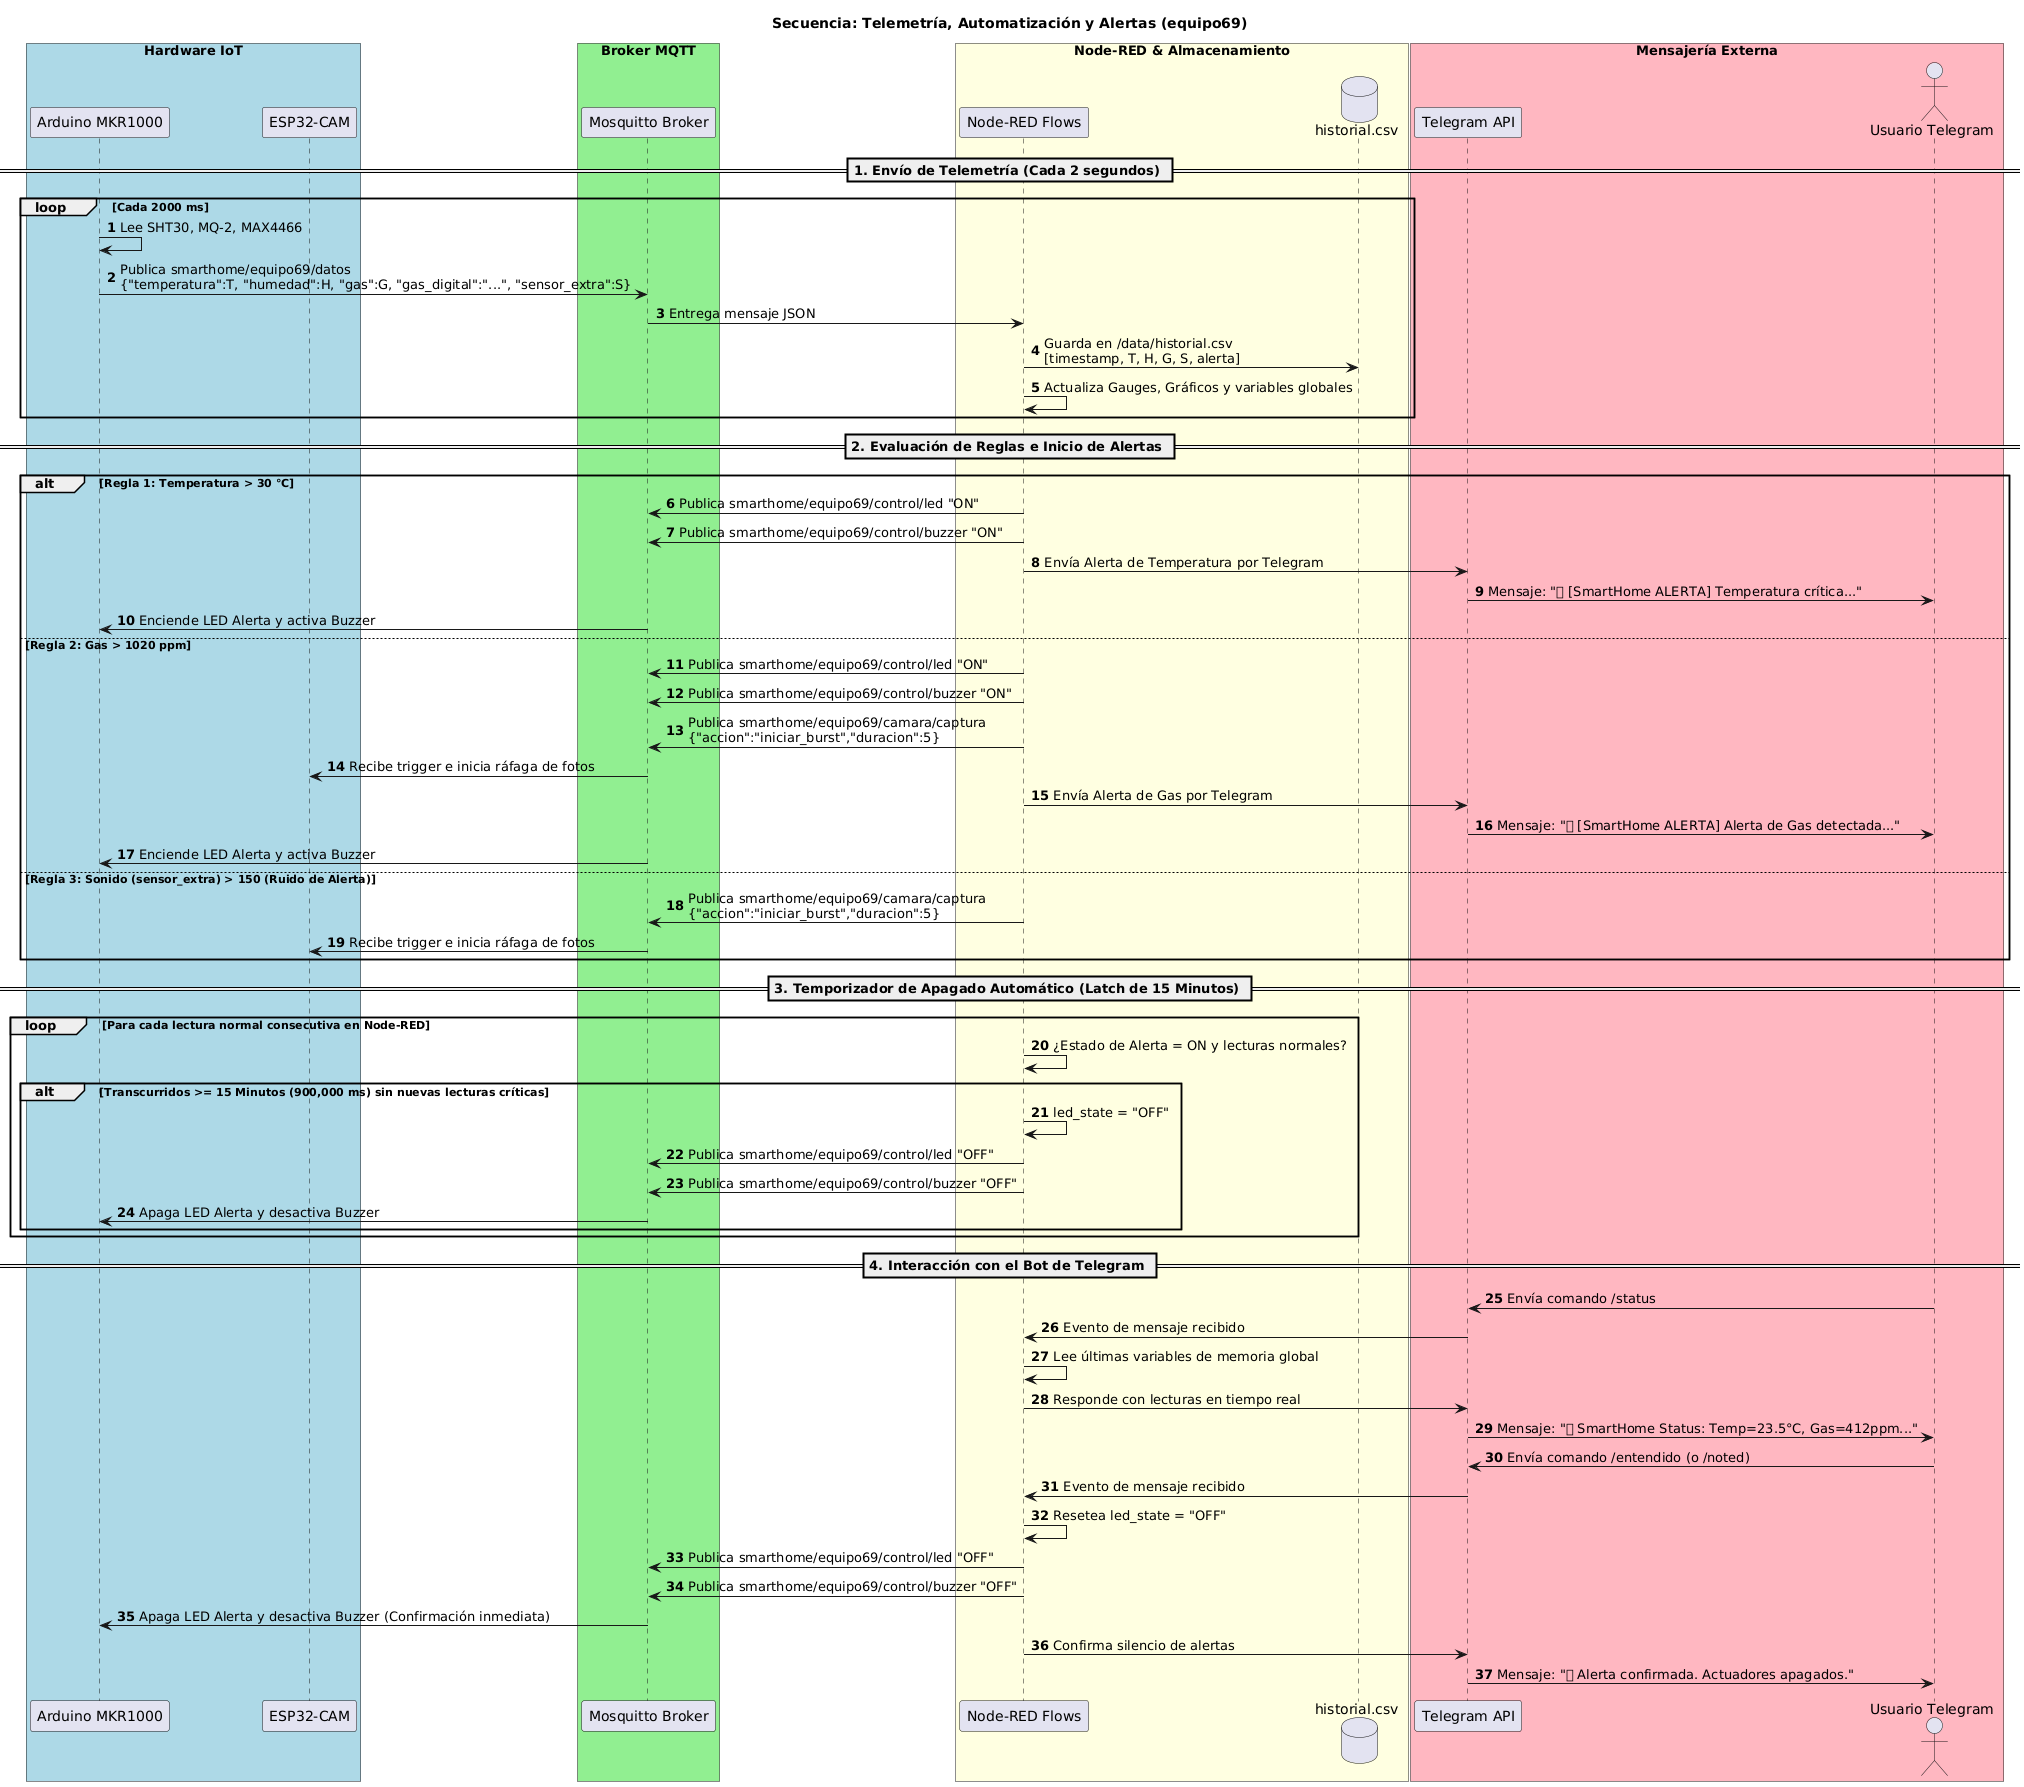
\includegraphics[width=0.75\textwidth]{arqui_3}}
    \caption{Diagrama de Secuencia de Monitoreo de Telemetría y Alertas Automáticas (arqui\_3). Al hacer clic en la imagen se abrirá el SVG de PlantUML en alta resolución.}
    \label{fig:arqui_secuencia_telemetria}
\end{figure}

% ==========================================
% 4. INVENTARIO E INTEGRACIÓN DE SENSORES
% ==========================================
\newpage
\section{Inventario e Integración de Sensores y Actuadores}

\subsection{Descripción de los Sensores y su Rol}
Para lograr un monitoreo completo del entorno y garantizar el correcto funcionamiento del control de accesos, se han integrado los siguientes dispositivos:
\begin{enumerate}
    \item \textbf{Sensor de Temperatura y Humedad SHT30 (I2C)}: Conectado a los pines de hardware dedicados I2C (SDA Pin 11, SCL Pin 12) del Arduino MKR1000. Su rol es proveer mediciones precisas del estado térmico y humedad del aire, variables esenciales para el confort y la detección de incendios o sobrecalentamiento de espacios.
    \item \textbf{Sensor de Gas Licuado y Humo MQ-2 (Analógico/Digital)}: Dispositivo electroquímico que mide la concentración de gases combustibles en el aire. Conectado al pin analógico \texttt{A0} para monitorear el nivel absoluto de gas y al pin digital \texttt{A2} como entrada de disparo rápida basada en el comparador del propio sensor físico. Su rol es emitir alertas críticas ante fugas o presencia de fuego.
    \item \textbf{Micrófono y Amplificador MAX4466 (Sonido - Analógico)}: Conectado al pin analógico \texttt{A1}. Mide las ondas de presión acústica realizando un muestreo continuo de pico a pico durante 50 milisegundos para determinar la amplitud del sonido ambiente. Actúa como sensor diferencial complementario, configurado como disparador acústico del sistema de seguridad.
    \item \textbf{Módulo de Cámara ESP32-CAM}: Tarjeta con microcontrolador ESP32-S y sensor OV2640. Su rol exclusivo es capturar y codificar imágenes JPEG bajo demanda tras recibir órdenes del bus MQTT, permitiendo al sistema de visión artificial en FastAPI realizar reconocimiento de personas en el hogar.
\end{enumerate}

\subsection{Actuadores}
El sistema cuenta con actuadores para señalización y respuesta física inmediata:
\begin{itemize}
    \item \textbf{LED de Alerta General (Pin 6)}: LED amarillo que se activa de forma continua al detectarse temperaturas críticas o niveles altos de gas licuado.
    \item \textbf{Buzzer de Alerta General (Pin 5)}: Generador de tonos sonoros para llamar la atención en la vivienda ante alarmas de seguridad activas.
    \item \textbf{LED Indicador de Puerta (Pin 8)}: LED verde que simula la cerradura eléctrica de acceso. Se enciende por 3 segundos tras verificarse la identidad de un habitante autorizado.
\end{itemize}

\subsection{Inventario Físico de Componentes}
El Cuadro \ref{tab:inventario_placas} y el Cuadro \ref{tab:inventario_componentes} detallan el stock físico utilizado en el prototipo de laboratorio.

\begin{table}[H]
    \centering
    \caption{Inventario de Placas de Desarrollo y Sensores}
    \label{tab:inventario_placas}
    \begin{tabular}{llcc}
        \toprule
        \textbf{Componente} & \textbf{Modelo/Descripción} & \textbf{Voltaje de Trabajo} & \textbf{Cantidad} \\
        \midrule
        Placa Principal & Arduino MKR1000 WiFi & 3.3 V (Micro USB) & 1 \\
        Cámara IoT & ESP32-CAM (con Shield MB) & 5.0 V (USB) & 1 \\
        Sensor Ambiental & SHT30 (Temperatura y Humedad) & 3.3 V & 1 \\
        Sensor de Gas & MQ-2 Gas/Humo & 5.0 V & 1 \\
        Micrófono/Sonido & MAX4466 con amplificador ajustable & 3.3 V & 1 \\
        \bottomrule
    \end{tabular}
\end{table}

\begin{table}[H]
    \centering
    \caption{Inventario de Componentes Pasivos y Accesorios}
    \label{tab:inventario_componentes}
    \begin{tabular}{llc}
        \toprule
        \textbf{Componente} & \textbf{Color / Detalle} & \textbf{Cantidad} \\
        \midrule
        Potenciómetros & Ajuste de ganancia y umbral & 4 \\
        LED de Alerta & Amarillo (Señalización de peligro) & 7 \\
        LED de Entrada & Verde (Simulador de electro-chapa) & 9 \\
        LED de Bloqueo & Rojo (Acceso Denegado) & 10 \\
        LED de Red & Azul (Estado de conexión WiFi) & 4 \\
        \bottomrule
    \end{tabular}
\end{table}

\subsection{Conexiones Físicas y Asignación de Pines}
La asignación de pines configurados en el firmware del Arduino MKR1000 (centralizados en \texttt{src/config.h}) se presenta en el Cuadro \ref{tab:pines_mkr}.

\begin{table}[H]
    \centering
    \caption{Asignación de Pines Físicos en el Arduino MKR1000}
    \label{tab:pines_mkr}
    \begin{tabular}{lccl}
        \toprule
        \textbf{Componente} & \textbf{Pin MKR1000} & \textbf{Dirección de Señal} & \textbf{Tipo de Señal} \\
        \midrule
        LED Alerta General & Pin 6 & Salida & Digital (PWM) \\
        Buzzer de Alerta & Pin 5 & Salida & Digital (PWM) \\
        LED Cerradura Puerta & Pin 8 & Salida & Digital (PWM) \\
        \midrule
        MQ-2 Analógico (AO) & Pin A0 & Entrada & Analógica (ADC) \\
        MQ-2 Digital (DO) & Pin A2 & Entrada & Digital \\
        MAX4466 Sonido (OUT) & Pin A1 & Entrada & Analógica (ADC) \\
        \midrule
        SHT30 Datos (SDA) & Pin 11 & Bidireccional & I2C Hardware Fijo \\
        SHT30 Reloj (SCL) & Pin 12 & Salida & I2C Hardware Fijo \\
        \bottomrule
    \end{tabular}
\end{table}

Las conexiones del sensor SHT30 se identifican mediante un cableado de cuatro hilos estructurado por colores normalizados: cable rojo para VCC (3.3V), cable negro para GND, cable verde para la línea SDA (Pin 11) y cable amarillo para la línea SCL (Pin 12).

% ==========================================
% 5. COMUNICACIÓN MQTT Y ESTRUCTURA DE TÓPICOS
% ==========================================
\newpage
\section{Comunicación MQTT y Estructura de Tópicos}
La mensajería MQTT (Message Queuing Telemetry Transport) es el núcleo de comunicación del sistema domótico. Se utiliza un broker Mosquitto configurado de forma aislada en Docker Compose accesible localmente a través del puerto estándar \texttt{1883}.

\subsection{Jerarquía de Tópicos Requerida}
Todos los tópicos del proyecto se estructuran bajo una jerarquía jerárquica limpia que utiliza el identificador del equipo asignado (\texttt{equipo69}) como namespace central. Esto garantiza la separación de mensajes en el caso de compartir un broker común. La estructura detallada se resume en el Cuadro \ref{tab:topicos_mqtt}.

\begin{table}[H]
    \centering
    \caption{Estructura de Tópicos MQTT del Sistema (Namespace: smarthome/equipo69/)}
    \label{tab:topicos_mqtt}
    \begin{tabular}{lcccl}
        \toprule
        \textbf{Tópico Relativo} & \textbf{Dirección} & \textbf{QoS} & \textbf{Retain} & \textbf{Propósito} \\
        \midrule
        \texttt{datos} & MKR $\rightarrow$ Broker & 0 & No & Envío de JSON con telemetría general \\
        \texttt{alerta} & MKR $\rightarrow$ Broker & 1 & No & Texto plano indicando alarma crítica \\
        \texttt{control/led} & Broker $\rightarrow$ MKR & 1 & Sí & Comando ``ON''/``OFF'' para LED de alerta \\
        \texttt{control/buzzer} & Broker $\rightarrow$ MKR & 1 & Sí & Comando ``ON''/``OFF'' para el Buzzer \\
        \texttt{control/led-puerta} & Broker $\rightarrow$ MKR & 1 & Sí & JSON para encender/apagar la cerradura \\
        \texttt{camara/evento} & ESP $\rightarrow$ Broker & 1 & No & JSON indicando estado de la cámara \\
        \texttt{camara/captura} & API $\rightarrow$ ESP & 1 & No & JSON ordenando ráfaga de fotos \\
        \texttt{camara/imagen} & ESP $\rightarrow$ Broker & 1 & No & Datos binarios de imágenes (JPEG) \\
        \texttt{acceso/estado} & API $\rightarrow$ Broker & 1 & No & JSON con veredicto de reconocimiento \\
        \texttt{acceso/enrolar} & API $\rightarrow$ Broker & 1 & No & JSON notificando ventana de enrolamiento \\
        \bottomrule
    \end{tabular}
\end{table}

\subsection{Formatos de Mensaje JSON}
Para simplificar el procesamiento en Node-RED y el backend FastAPI, los datos de sensores del Arduino MKR1000 se empaquetan en un único documento JSON estructurado que se publica de forma asíncrona cada 2 segundos. Si algún sensor físico experimenta una falla o desconexión, la clave asociada toma un valor nulo de manera explícita (en lugar de enviar $0.0$, cumpliendo con las especificaciones técnicas).

El listado \ref{lst:json_telemetria} muestra un ejemplo real del mensaje JSON publicado en el tópico \texttt{smarthome/equipo69/datos} bajo condiciones de operación normal.

\begin{lstlisting}[language=json, label=lst:json_telemetria, caption={Ejemplo de payload JSON publicado por el nodo de sensores.}]
{
  "equipo": "equipo69",
  "temperatura": 23.5,
  "humedad": 61.2,
  "gas": 412,
  "gas_digital": "NORMAL",
  "sensor_extra": 128
}
\end{lstlisting}

En caso de que el sensor ambiental SHT30 falle o esté desconectado eléctricamente, el JSON se reestructura automáticamente omitiendo los valores erróneos o reemplazándolos por valores nulos, tal como se ilustra en el Listado \ref{lst:json_falla}.

\begin{lstlisting}[language=json, label=lst:json_falla, caption={Ejemplo de payload JSON bajo falla del sensor SHT30.}]
{
  "equipo": "equipo69",
  "temperatura": null,
  "humedad": null,
  "gas": 415,
  "gas_digital": "NORMAL",
  "sensor_extra": 130
}
\end{lstlisting}

El comando para accionar la puerta enviado al tópico \texttt{smarthome/equipo69/control/led-puerta} utiliza la estructura: \texttt{\{"accion": "ON"\}} o \texttt{\{"accion": "OFF"\}}. Por otro lado, la orden de ráfaga a la cámara en el tópico \texttt{smarthome/equipo69/camara/captura} utiliza: \texttt{\{"accion": "iniciar\_burst", "duracion": 5\}}.

% ==========================================
% 6. ESTRATEGIAS DE CONTROL AUTOMÁTICO
% ==========================================
\newpage
\section{Estrategias de Control Automático y Notificaciones}
El sistema implementa una lógica de control de bucle cerrado basada en reglas de decisión programadas en Node-RED y en el backend FastAPI, respondiendo de manera autónoma ante emergencias.

\subsection{Reglas de Automatización de Emergencias}
Las tres estrategias principales de control automático implementadas en Node-RED son:
\begin{enumerate}
    \item \textbf{Control por Temperatura Crítica}: Si la lectura analizada de temperatura supera los $30^{\circ}\text{C}$, Node-RED publica comandos ``ON'' independientes a los tópicos de control de actuadores locales (\texttt{control/led} y \texttt{control/buzzer}), y genera un mensaje con formato Markdown enriquecido dirigido al bot de Telegram. La alarma permanece activa hasta que la lectura disminuya de los $30^{\circ}\text{C}$ y transcurra el tiempo de enclavamiento.
    \item \textbf{Control por Gas Crítico}: Cuando el valor analógico del MQ-2 supera las $1020$ ppm (o la entrada digital DO pasa a nivel \texttt{LOW}), se asume la presencia de gases combustibles nocivos. Node-RED activa de forma inmediata el LED de alerta y el buzzer, ordena a la cámara capturar una ráfaga mediante la publicación en \texttt{camara/captura}, y despacha una alerta roja por Telegram indicando la concentración exacta detectada.
    \item \textbf{Disparo de Seguridad por Ruido Fuerte (MAX4466)}: El sensor de sonido de pico a pico (\texttt{sensor\_extra}) actúa como centinela en la noche. Si el nivel acústico sobrepasa el umbral dinámico de $150$ unidades, el sistema infiere un evento sospechoso (ej. golpe o rotura de cristal) y gatilla automáticamente una orden de ráfaga a la cámara ESP32-CAM. Las imágenes se procesan de inmediato en busca de rostros.
\end{enumerate}

\subsection{Prevención de Alertas Repetitivas (Cooldown) y Enclavamiento}
Para evitar la saturación de los canales de comunicación externos y proteger la tranquilidad de la familia, se han integrado mecanismos de software en los flujos de Node-RED:
\begin{itemize}
    \item \textbf{Cooldown de Notificaciones}: Cuando una regla crítica se dispara, se genera una notificación externa y se almacena la hora del envío en la memoria temporal de Node-RED (\texttt{flow.set("lastAlertTime", Date.now())}). El sistema bloquea nuevos despachos por Telegram durante los siguientes 60 segundos, aunque la variable crítica siga por encima del umbral.
    \item \textbf{Latching (Retención) y Temporizador de 15 Minutos}: A nivel físico, un LED oscilando rápidamente debido a variaciones de ruido de los sensores genera desgaste y fatiga. Si los sensores vuelven a rangos seguros, el LED y el buzzer no se apagan inmediatamente. Node-RED mantiene el estado ``ON'' por un mínimo de 15 minutos ($900.000$ milisegundos) desde el último valor crítico leído. Este temporizador se evalúa de manera asíncrona no bloqueante utilizando comparaciones de tiempo en milisegundos (\texttt{millis()}).
\end{itemize}

% ==========================================
% 7. DASHBOARD Y INTERFACES
% ==========================================
\newpage
\section{Dashboard y Canales de Interfaz}

\subsection{Panel de Monitoreo Node-RED Dashboard}
La interfaz de usuario principal de Node-RED se sirve en la URL \texttt{http://localhost:1880/ui} y contiene widgets interactivos organizados en tres grupos:
\begin{itemize}
    \item \textbf{Sensores en Tiempo Real}: Dos relojes analógicos de aguja (Gauges) para Temperatura ($0\text{--}50^{\circ}\text{C}$) y Humedad ($0\text{--}100\%$), un indicador tipo brújula de ppm de Gas MQ-2 ($0\text{--}1024$), y un campo de texto dinámico que muestra la intensidad acústica del MAX4466.
    \item \textbf{Seguridad e Imagen de Cámara}: Un widget de plantilla HTML que despliega en Base64 la última fotografía transmitida por la ESP32-CAM, un indicador circular de estado (verde para estado normal, rojo para alerta de intrusión o emergencia) y texto descriptivo de rostros detectados.
    \item \textbf{Controles Manuales e Historial}: Botones virtuales para encender y silenciar manualmente el LED y el buzzer de alerta, y un gráfico de líneas dinámico que despliega la curva histórica de temperatura de las últimas 5 horas.
\end{itemize}

\subsection{Interfaz Web de Acceso Personalizada}
El sistema cuenta con un segundo frontend especializado en control de accesos desarrollado en vanilla HTML5/JS y servido por Nginx en el puerto \texttt{80}. Este panel consulta la API REST de FastAPI mediante polling cada 2 segundos. Muestra la cámara en vivo relay a través de un stream MJPEG dinámico, visualiza una tabla ordenada con el historial de accesos reciente extraído de la base de datos y despliega el formulario temporal de enrolamiento para registrar rostros detectados como desconocidos.

\subsection{Bot de Telegram}
El bot de Telegram (\texttt{SmartHomeBot}) implementa comandos bidireccionales administrados por Node-RED:
\begin{itemize}
    \item \texttt{/status}: Responde inmediatamente con un mensaje estructurado detallando las lecturas más recientes almacenadas en el contexto global del sistema (Temperatura, Humedad, Gas y Sonido).
    \item \texttt{/ayuda} o \texttt{/start}: Despliega el menú interactivo con la descripción de los comandos soportados.
    \item \texttt{/entendido} o \texttt{/noted}: Comando prioritario de confirmación de alerta. Permite al propietario apagar de forma remota y segura los actuadores de emergencia (LED de Alerta y Buzzer) antes de que venza el enclavamiento de 15 minutos en Node-RED.
\end{itemize}

\subsection{Registro Histórico de Datos}
La persistencia de la telemetría e incidentes del sistema se asegura en dos niveles:
\begin{enumerate}
    \item \textbf{Historial Ambiental (CSV)}: Node-RED concatena cada lectura en una cadena separada por comas con formato: \texttt{timestamp,temperatura,humedad,gas,sensor\_extra,alerta}. Los datos se escriben recursivamente en el archivo plano \texttt{/data/historial.csv}, persistido de forma segura en el host a través de un bind mount del contenedor Docker.
    \item \textbf{Historial de Accesos (SQLite)}: El backend FastAPI gestiona la base de datos SQLite \texttt{access\_control.db}. Esta almacena en la tabla \texttt{usuarios} la identidad de las personas autorizadas junto con el blob serializado de su firma facial de 128 dimensiones. La tabla \texttt{historial} registra cada evento de la puerta principal (``Entrada Automática'', ``Apertura Manual'', ``Desconocido Detectado'' o ``Sin Rostro'') junto con su respectiva marca temporal en hora chilena.
\end{enumerate}

% ==========================================
% 8. PROBLEMAS ENCONTRADOS Y SOLUCIONES
% ==========================================
\newpage
\section{Problemas Encontrados y Soluciones Aplicadas}
Durante las pruebas de integración del sistema distribuido con hardware físico, surgieron tres problemas complejos que requirieron optimizaciones avanzadas de software.

\subsection{Problema 1: Apagado Inexistente del LED de Alerta}
\textbf{Descripción}: Originalmente, el LED y el buzzer de alerta se activaban de forma correcta al detectarse una variable crítica en Node-RED, pero permanecían encendidos de forma indefinida hasta que se enviaba un comando manual desde Telegram o el dashboard. Esto presentaba un riesgo de sobrecalentamiento de actuadores y contaminación acústica ante falsas alarmas temporales. \\
\textbf{Solución}: Se programó un contador de tiempo lógico en Node-RED utilizando variables de flujo (\texttt{flow.get("lastAlertTime")}). Ahora, cada vez que una lectura supera los límites, se refresca la marca temporal del evento. Si los sensores retornan a valores normales, el flujo ejecuta una verificación periódica. Tras transcurrir 15 minutos ($900.000$ ms) consecutivos sin lecturas críticas en el bus, Node-RED publica de forma automática comandos ``OFF'' a los actuadores para normalizar el hogar sin requerir intervención del usuario.

\subsection{Problema 2: Inestabilidad y Pérdida en el Reconocimiento Facial}
\textbf{Descripción}: La visión artificial experimentaba tres fallas severas: (a) El reconocimiento fallaba frecuentemente por cambios en las condiciones de luz natural en el acceso. (b) Las imágenes transmitidas por MQTT aparecían cortadas o con líneas grises debido al choque de paquetes de red al transmitir streams continuos pesados. (c) La tasa de falsos rechazos era muy alta debido a límites de tolerancia extremadamente rígidos en el algoritmo. Además, si el sensor MAX4466 enviaba múltiples picos de sonido seguidos, se disparaban ráfagas de fotos concurrentes sin pausar, saturando el broker y bloqueando la evaluación del backend. \\
\textbf{Solución}: Se realizaron las siguientes modificaciones correctoras en el backend de FastAPI y en el firmware:
\begin{enumerate}
    \item Se eliminó el servidor HTTP de streaming local de la ESP32-CAM. Ahora la cámara trabaja de forma pasiva enviando únicamente ráfagas de fotos controladas por MQTT tras recibir el evento de captura.
    \item Se redujo el tamaño del burst de frames en la ESP32-CAM: ahora captura y transmite ráfagas cortas de 3 a 5 imágenes espaciadas por 250ms en lugar del esquema anterior de 10 frames continuos de video. Esto mitigó el choque de paquetes de red y solucionó la corrupción de imágenes JPEG.
    \item Se implementaron parámetros de comparación flexibles en el archivo del backend \texttt{processor.py}: la tolerancia geométrica se redujo a \texttt{0.35} (haciendo el emparejamiento de vectores de distancia dlib más selectivo y seguro) y la confianza mínima se fijó en \texttt{0.50}. Para robustecer la decisión, el sistema requiere confirmación en al menos 3 frames consecutivos del burst para dar por válida la identidad del usuario.
    \item En el backend FastAPI, se introdujo un semáforo asíncrono global (\texttt{\_capture\_lock = asyncio.Lock()}) y un flag de captura en el estado de la aplicación (\texttt{app.state.capturing}). Si se detectan múltiples eventos acústicos seguidos, el backend ignora las peticiones adicionales mientras una sesión de captura de 10 segundos esté activa, evitando la superposición de tareas.
\end{enumerate}

\subsection{Problema 3: Caídas Frecuentes a Cero del Sensor de Gas MQ-2}
\textbf{Descripción}: El sensor MQ-2 presentó un comportamiento físico anómalo: al exponerse a altas concentraciones de gas licuado o humo denso que superaban el rango máximo nominal del sensor, la lectura analizada en el MKR1000 se saturaba y caía abruptamente a 0 de forma momentánea antes de recuperarse. En el código original de control automático, esto provocaba que el sistema interpretara la caída a 0 como un retorno a la normalidad y apagara inmediatamente los actuadores de alerta, provocando un parpadeo intermitente peligroso en medio de una fuga real. \\
\textbf{Solución}: Este fallo físico se resolvió por software a través de dos estrategias combinadas en el flujo de Node-RED:
\begin{enumerate}
    \item \textbf{Ajuste del Umbral Crítico}: Se configuró el umbral de alarma de gas (\texttt{gas\_threshold}) en el valor máximo seguro de \texttt{1020} ppm (dentro de un rango de ADC de 10 bits de 0 a 1023). Al ubicar el umbral justo al borde de la saturación del sensor, se garantiza que la alarma se active inmediatamente antes de que ocurra la caída física del voltaje.
    \item \textbf{Lógica de Latch y Evaluación Condicional}: En el nodo \texttt{rules\_evaluator} de Node-RED, la lógica de alarma se evalúa de manera condicionada mediante la sentencia \texttt{if (gas \&\& gas > gasThreshold)}. En Javascript, el valor 0 se evalúa como falso (\emph{falsy}), por lo que si el sensor cae a 0, la regla de activación no se ejecuta de nuevo. Sin embargo, debido al enclavamiento (latch) por software implementado con la variable global de tiempo \texttt{flow.set("lastAlertTime", Date.now())}, el estado de alerta general permanece en ``ON'' y no apaga los actuadores. Node-RED requiere que pasen 15 minutos consecutivos con lecturas estrictamente válidas y por debajo del umbral para enviar la orden de apagado. De este modo, las caídas transitorias a 0 son ignoradas por el sistema físico de advertencia.
\end{enumerate}

% ==========================================
% 9. CONCLUSIONES
% ==========================================
\newpage
\section{Conclusiones}
La implementación de este prototipo domótico de SmartHome IoT demuestra el valor de las arquitecturas modulares y distribuidas para la automatización de viviendas. Mediante el uso de un bus de datos MQTT centralizado, se logró desacoplar las tareas de lectura física y actuación (MKR1000) de los procesos computacionalmente intensivos como el reconocimiento facial (FastAPI) y la orquestación del dashboard web junto con la lógica de control (Node-RED).

Entre las principales lecciones técnicas obtenidas se destaca la importancia de diseñar sistemas de tolerancia a fallos por software para mitigar las limitaciones físicas inherentes del hardware económico. La inestabilidad en las lecturas del sensor de gas MQ-2 o la saturación de corriente por ráfagas concurrentes en la cámara demostraron que la programación basada puramente en estados instantáneos de sensores es insuficiente para entornos críticos de seguridad. La incorporación de técnicas de enclavamiento temporal (latch), filtros de concurrencia mediante cerrojos de exclusión mutua (\texttt{Locks}) y la calibración fina de umbrales permitieron transformar componentes inestables en una solución robusta y confiable.

Como trabajo futuro, se recomienda la transición del protocolo de red a conexiones con seguridad TLS y autenticación por usuario/contraseña en Mosquitto, la integración de un esquema de alimentación ininterrumpida (UPS) para prevenir caídas ante cortes de suministro eléctrico, y la implementación de técnicas de aprendizaje federado para entrenar el modelo de visión artificial localmente con mayor cantidad de imágenes de muestra ante condiciones adversas de iluminación.

\end{document}
